
%% bare_conf.tex
%% V1.3
%% 2007/01/11
%% by Michael Shell
%% See:
%% http://www.michaelshell.org/
%% for current contact information.
%%
%% This is a skeleton file demonstrating the use of IEEEtran.cls
%% (requires IEEEtran.cls version 1.7 or later) with an IEEE conference paper.
%%
%% Support sites:
%% http://www.michaelshell.org/tex/ieeetran/
%% http://www.ctan.org/tex-archive/macros/latex/contrib/IEEEtran/
%% and
%% http://www.ieee.org/

%%*************************************************************************
%% Legal Notice:
%% This code is offered as-is without any warranty either expressed or
%% implied; without even the implied warranty of MERCHANTABILITY or
%% FITNESS FOR A PARTICULAR PURPOSE! 
%% User assumes all risk.
%% In no event shall IEEE or any contributor to this code be liable for
%% any damages or losses, including, but not limited to, incidental,
%% consequential, or any other damages, resulting from the use or misuse
%% of any information contained here.
%%
%% All comments are the opinions of their respective authors and are not
%% necessarily endorsed by the IEEE.
%%
%% This work is distributed under the LaTeX Project Public License (LPPL)
%% ( http://www.latex-project.org/ ) version 1.3, and may be freely used,
%% distributed and modified. A copy of the LPPL, version 1.3, is included
%% in the base LaTeX documentation of all distributions of LaTeX released
%% 2003/12/01 or later.
%% Retain all contribution notices and credits.
%% ** Modified files should be clearly indicated as such, including  **
%% ** renaming them and changing author support contact information. **
%%
%% File list of work: IEEEtran.cls, IEEEtran_HOWTO.pdf, bare_adv.tex,
%%                    bare_conf.tex, bare_jrnl.tex, bare_jrnl_compsoc.tex
%%*************************************************************************

% *** Authors should verify (and, if needed, correct) their LaTeX system  ***
% *** with the testflow diagnostic prior to trusting their LaTeX platform ***
% *** with production work. IEEE's font choices can trigger bugs that do  ***
% *** not appear when using other class files.                            ***
% The testflow support page is at:
% http://www.michaelshell.org/tex/testflow/



% Note that the a4paper option is mainly intended so that authors in
% countries using A4 can easily print to A4 and see how their papers will
% look in print - the typesetting of the document will not typically be
% affected with changes in paper size (but the bottom and side margins will).
% Use the testflow package mentioned above to verify correct handling of
% both paper sizes by the user's LaTeX system.
%
% Also note that the "draftcls" or "draftclsnofoot", not "draft", option
% should be used if it is desired that the figures are to be displayed in
% draft mode.
%
\documentclass[conference]{IEEEtran}
% Add the compsoc option for Computer Society conferences.
%
% If IEEEtran.cls has not been installed into the LaTeX system files,
% manually specify the path to it like:
% \documentclass[conference]{../sty/IEEEtran}





% Some very useful LaTeX packages include:
% (uncomment the ones you want to load)


% *** MISC UTILITY PACKAGES ***
%
%\usepackage{ifpdf}
% Heiko Oberdiek's ifpdf.sty is very useful if you need conditional
% compilation based on whether the output is pdf or dvi.
% usage:
% \ifpdf
%   % pdf code
% \else
%   % dvi code
% \fi
% The latest version of ifpdf.sty can be obtained from:
% http://www.ctan.org/tex-archive/macros/latex/contrib/oberdiek/
% Also, note that IEEEtran.cls V1.7 and later provides a builtin
% \ifCLASSINFOpdf conditional that works the same way.
% When switching from latex to pdflatex and vice-versa, the compiler may
% have to be run twice to clear warning/error messages.






% *** CITATION PACKAGES ***
%
\usepackage{cite}
% cite.sty was written by Donald Arseneau
% V1.6 and later of IEEEtran pre-defines the format of the cite.sty package
% \cite{} output to follow that of IEEE. Loading the cite package will
% result in citation numbers being automatically sorted and properly
% "compressed/ranged". e.g., [1], [9], [2], [7], [5], [6] without using
% cite.sty will become [1], [2], [5]--[7], [9] using cite.sty. cite.sty's
% \cite will automatically add leading space, if needed. Use cite.sty's
% noadjust option (cite.sty V3.8 and later) if you want to turn this off.
% cite.sty is already installed on most LaTeX systems. Be sure and use
% version 4.0 (2003-05-27) and later if using hyperref.sty. cite.sty does
% not currently provide for hyperlinked citations.
% The latest version can be obtained at:
% http://www.ctan.org/tex-archive/macros/latex/contrib/cite/
% The documentation is contained in the cite.sty file itself.






% *** GRAPHICS RELATED PACKAGES ***
%
\ifCLASSINFOpdf
  \usepackage[pdftex]{graphicx}
  % declare the path(s) where your graphic files are
  % \graphicspath{{../pdf/}{../jpeg/}}
  % and their extensions so you won't have to specify these with
  % every instance of \includegraphics
  % \DeclareGraphicsExtensions{.pdf,.jpeg,.png}
\else
  % or other class option (dvipsone, dvipdf, if not using dvips). graphicx
  % will default to the driver specified in the system graphics.cfg if no
  % driver is specified.
  \usepackage[dvips]{graphicx}
  % declare the path(s) where your graphic files are
  % \graphicspath{{../eps/}}
  % and their extensions so you won't have to specify these with
  % every instance of \includegraphics
  % \DeclareGraphicsExtensions{.eps}
\fi
% graphicx was written by David Carlisle and Sebastian Rahtz. It is
% required if you want graphics, photos, etc. graphicx.sty is already
% installed on most LaTeX systems. The latest version and documentation can
% be obtained at: 
% http://www.ctan.org/tex-archive/macros/latex/required/graphics/
% Another good source of documentation is "Using Imported Graphics in
% LaTeX2e" by Keith Reckdahl which can be found as epslatex.ps or
% epslatex.pdf at: http://www.ctan.org/tex-archive/info/
%
% latex, and pdflatex in dvi mode, support graphics in encapsulated
% postscript (.eps) format. pdflatex in pdf mode supports graphics
% in .pdf, .jpeg, .png and .mps (metapost) formats. Users should ensure
% that all non-photo figures use a vector format (.eps, .pdf, .mps) and
% not a bitmapped formats (.jpeg, .png). IEEE frowns on bitmapped formats
% which can result in "jaggedy"/blurry rendering of lines and letters as
% well as large increases in file sizes.
%
% You can find documentation about the pdfTeX application at:
% http://www.tug.org/applications/pdftex





% *** MATH PACKAGES ***
%
%\usepackage[cmex10]{amsmath}
% A popular package from the American Mathematical Society that provides
% many useful and powerful commands for dealing with mathematics. If using
% it, be sure to load this package with the cmex10 option to ensure that
% only type 1 fonts will utilized at all point sizes. Without this option,
% it is possible that some math symbols, particularly those within
% footnotes, will be rendered in bitmap form which will result in a
% document that can not be IEEE Xplore compliant!
%
% Also, note that the amsmath package sets \interdisplaylinepenalty to 10000
% thus preventing page breaks from occurring within multiline equations. Use:
%\interdisplaylinepenalty=2500
% after loading amsmath to restore such page breaks as IEEEtran.cls normally
% does. amsmath.sty is already installed on most LaTeX systems. The latest
% version and documentation can be obtained at:
% http://www.ctan.org/tex-archive/macros/latex/required/amslatex/math/





% *** SPECIALIZED LIST PACKAGES ***
%
%\usepackage{algorithmic}
% algorithmic.sty was written by Peter Williams and Rogerio Brito.
% This package provides an algorithmic environment fo describing algorithms.
% You can use the algorithmic environment in-text or within a figure
% environment to provide for a floating algorithm. Do NOT use the algorithm
% floating environment provided by algorithm.sty (by the same authors) or
% algorithm2e.sty (by Christophe Fiorio) as IEEE does not use dedicated
% algorithm float types and packages that provide these will not provide
% correct IEEE style captions. The latest version and documentation of
% algorithmic.sty can be obtained at:
% http://www.ctan.org/tex-archive/macros/latex/contrib/algorithms/
% There is also a support site at:
% http://algorithms.berlios.de/index.html
% Also of interest may be the (relatively newer and more customizable)
% algorithmicx.sty package by Szasz Janos:
% http://www.ctan.org/tex-archive/macros/latex/contrib/algorithmicx/




% *** ALIGNMENT PACKAGES ***
%
%\usepackage{array}
% Frank Mittelbach's and David Carlisle's array.sty patches and improves
% the standard LaTeX2e array and tabular environments to provide better
% appearance and additional user controls. As the default LaTeX2e table
% generation code is lacking to the point of almost being broken with
% respect to the quality of the end results, all users are strongly
% advised to use an enhanced (at the very least that provided by array.sty)
% set of table tools. array.sty is already installed on most systems. The
% latest version and documentation can be obtained at:
% http://www.ctan.org/tex-archive/macros/latex/required/tools/


%\usepackage{mdwmath}
%\usepackage{mdwtab}
% Also highly recommended is Mark Wooding's extremely powerful MDW tools,
% especially mdwmath.sty and mdwtab.sty which are used to format equations
% and tables, respectively. The MDWtools set is already installed on most
% LaTeX systems. The lastest version and documentation is available at:
% http://www.ctan.org/tex-archive/macros/latex/contrib/mdwtools/


% IEEEtran contains the IEEEeqnarray family of commands that can be used to
% generate multiline equations as well as matrices, tables, etc., of high
% quality.


%\usepackage{eqparbox}
% Also of notable interest is Scott Pakin's eqparbox package for creating
% (automatically sized) equal width boxes - aka "natural width parboxes".
% Available at:
% http://www.ctan.org/tex-archive/macros/latex/contrib/eqparbox/





% *** SUBFIGURE PACKAGES ***
%\usepackage[tight,footnotesize]{subfigure}
% subfigure.sty was written by Steven Douglas Cochran. This package makes it
% easy to put subfigures in your figures. e.g., "Figure 1a and 1b". For IEEE
% work, it is a good idea to load it with the tight package option to reduce
% the amount of white space around the subfigures. subfigure.sty is already
% installed on most LaTeX systems. The latest version and documentation can
% be obtained at:
% http://www.ctan.org/tex-archive/obsolete/macros/latex/contrib/subfigure/
% subfigure.sty has been superceeded by subfig.sty.



%\usepackage[caption=false]{caption}
%\usepackage[font=footnotesize]{subfig}
% subfig.sty, also written by Steven Douglas Cochran, is the modern
% replacement for subfigure.sty. However, subfig.sty requires and
% automatically loads Axel Sommerfeldt's caption.sty which will override
% IEEEtran.cls handling of captions and this will result in nonIEEE style
% figure/table captions. To prevent this problem, be sure and preload
% caption.sty with its "caption=false" package option. This is will preserve
% IEEEtran.cls handing of captions. Version 1.3 (2005/06/28) and later 
% (recommended due to many improvements over 1.2) of subfig.sty supports
% the caption=false option directly:
%\usepackage[caption=false,font=footnotesize]{subfig}
%
% The latest version and documentation can be obtained at:
% http://www.ctan.org/tex-archive/macros/latex/contrib/subfig/
% The latest version and documentation of caption.sty can be obtained at:
% http://www.ctan.org/tex-archive/macros/latex/contrib/caption/




% *** FLOAT PACKAGES ***
%
%\usepackage{fixltx2e}
% fixltx2e, the successor to the earlier fix2col.sty, was written by
% Frank Mittelbach and David Carlisle. This package corrects a few problems
% in the LaTeX2e kernel, the most notable of which is that in current
% LaTeX2e releases, the ordering of single and double column floats is not
% guaranteed to be preserved. Thus, an unpatched LaTeX2e can allow a
% single column figure to be placed prior to an earlier double column
% figure. The latest version and documentation can be found at:
% http://www.ctan.org/tex-archive/macros/latex/base/



%\usepackage{stfloats}
% stfloats.sty was written by Sigitas Tolusis. This package gives LaTeX2e
% the ability to do double column floats at the bottom of the page as well
% as the top. (e.g., "\begin{figure*}[!b]" is not normally possible in
% LaTeX2e). It also provides a command:
%\fnbelowfloat
% to enable the placement of footnotes below bottom floats (the standard
% LaTeX2e kernel puts them above bottom floats). This is an invasive package
% which rewrites many portions of the LaTeX2e float routines. It may not work
% with other packages that modify the LaTeX2e float routines. The latest
% version and documentation can be obtained at:
% http://www.ctan.org/tex-archive/macros/latex/contrib/sttools/
% Documentation is contained in the stfloats.sty comments as well as in the
% presfull.pdf file. Do not use the stfloats baselinefloat ability as IEEE
% does not allow \baselineskip to stretch. Authors submitting work to the
% IEEE should note that IEEE rarely uses double column equations and
% that authors should try to avoid such use. Do not be tempted to use the
% cuted.sty or midfloat.sty packages (also by Sigitas Tolusis) as IEEE does
% not format its papers in such ways.





% *** PDF, URL AND HYPERLINK PACKAGES ***
%
%\usepackage{url}
% url.sty was written by Donald Arseneau. It provides better support for
% handling and breaking URLs. url.sty is already installed on most LaTeX
% systems. The latest version can be obtained at:
% http://www.ctan.org/tex-archive/macros/latex/contrib/misc/
% Read the url.sty source comments for usage information. Basically,
% \url{my_url_here}.





% *** Do not adjust lengths that control margins, column widths, etc. ***
% *** Do not use packages that alter fonts (such as pslatex).         ***
% There should be no need to do such things with IEEEtran.cls V1.6 and later.
% (Unless specifically asked to do so by the journal or conference you plan
% to submit to, of course. )


% correct bad hyphenation here
\hyphenation{op-tical net-works semi-conduc-tor}

%%%%%%%%%%%%%%%%%%%%%%%%%%%%%%%%%%%%%%%%%%%%%%%%%%%%%%
\usepackage{tabulary} %tabla que ajusta celdas al texto
\usepackage{placeins} % ayuda a que las tablas no queden en medio de los textos
\usepackage[font={footnotesize}]{caption} % tamano para la descripcion de las tablas
\captionsetup{labelformat=empty} % elimina el prefijo de los nombres de las tablas
\renewcommand{\arraystretch}{1.3}
\renewcommand{\refname}{Referencias}
\renewcommand{\abstractname}{Resumen}
\usepackage{float}
\usepackage{makecell}
\usepackage{lipsum}
%%%%%%%%%%%%%%%%%%%%%%%%%%%%%%%%%%%%%%%%%%%%%%%%%%%%%%

\begin{document}
%
% paper title
% can use linebreaks \\ within to get better formatting as desired
\title{Software para el Espectrofot\'{o}metro ``MiniScan XE Plus'' usado en el Diagn\'{o}stico de Patolog\'{i}as Dermatol\'{o}gicas en Pacientes}


% author names and affiliations
% use a multiple column layout for up to three different
% affiliations

% conference papers do not typically use \thanks and this command
% is locked out in conference mode. If really needed, such as for
% the acknowledgment of grants, issue a \IEEEoverridecommandlockouts
% after \documentclass

% for over three affiliations, or if they all won't fit within the width
% of the page, use this alternative format:
% 
\author{\IEEEauthorblockN{Gabriel N\'{u}\~{n}ez\IEEEauthorrefmark{1},\IEEEauthorrefmark{4},\IEEEauthorrefmark{5},
Harold Vazques\IEEEauthorrefmark{1},\IEEEauthorrefmark{4},
Patricia Guerrero\IEEEauthorrefmark{1},\IEEEauthorrefmark{4}, y 
Aar\'{o}n Mu\~{n}oz\IEEEauthorrefmark{2},\IEEEauthorrefmark{3},\IEEEauthorrefmark{4}}
\IEEEauthorblockA{\IEEEauthorrefmark{1}Facultad Experimental de Ciencias y Tecnolog\'{i}a, Departamento de Computaci\'{o}n}
\IEEEauthorblockA{\IEEEauthorrefmark{2}Facultad Experimental de Ciencias y Tecnolog\'{i}a, Departamento de F\'{i}sica}
\IEEEauthorblockA{\IEEEauthorrefmark{3}Centro de Investigaciones M\'{e}dicas y Biotecnol\'{o}gicas de la Universidad de Carabobo}
\IEEEauthorblockA{\IEEEauthorrefmark{4}Universidad de Carabobo, Valencia, Venezuela}
\IEEEauthorblockA{\IEEEauthorrefmark{5}Email: gabriel.nzn@gmail.com}}




% use for special paper notices
%\IEEEspecialpapernotice{(Invited Paper)}




% make the title area
\maketitle


\begin{abstract}
%\boldmath
El Espectrofot\'{o}metro de reflexi\'{o}n difusa ``MiniScan XE Plus'' es un instrumento de medici\'{o}n utilizado por el Centro de Investigaciones M\'{e}dicas y Biotecnol\'{o}gicas de la Universidad de Carabobo (CIMBUC), el cual ayuda a los dermat\'{o}logos a establecer diagn\'{o}sticos sobre patolog\'{i}as en la piel de pacientes de manera precisa y sin necesidad de realizar biopsias. No obstante, el software disponible para la utilizaci\'{o}n de dicho instrumento es poco amigable, dificil de utilizar e imposible de modificar y extender. La presente investigaci\'{o}n tiene como objetivo desarrollar un nuevo software que se ajuste a las necesidades de los dermat\'{o}logos y que garantice un mejor aprovechamiento del instrumento en cuesti\'{o}n.
\end{abstract}
% IEEEtran.cls defaults to using nonbold math in the Abstract.
% This preserves the distinction between vectors and scalars. However,
% if the conference you are submitting to favors bold math in the abstract,
% then you can use LaTeX's standard command \boldmath at the very start
% of the abstract to achieve this. Many IEEE journals/conferences frown on
% math in the abstract anyway.

% no keywords




% For peer review papers, you can put extra information on the cover
% page as needed:
% \ifCLASSOPTIONpeerreview
% \begin{center} \bfseries EDICS Category: 3-BBND \end{center}
% \fi
%
% For peerreview papers, this IEEEtran command inserts a page break and
% creates the second title. It will be ignored for other modes.
\IEEEpeerreviewmaketitle

\section{Introducci\'{o}n}
% no \IEEEPARstart

La Espectroscop\'{i}a de Reflectancia Difusa es una t\'{e}cnica \'{o}ptica con la cual es  posible estudiar las propiedades bioqu\'{i}micas y las condiciones estructurales de un tejido biol\'{o}gico, analizando la interacci\'{o}n luz-tejido de una manera no invasiva \cite{Perez}. Durante el diagn\'{o}stico no invasivo no se crea ninguna ruptura en la piel, y los pacientes no se someten al dolor ni a cicatrices durante el tratamiento \cite{Bersha}.

En este sentido, el Centro de Investigaciones M\'{e}dicas y Biotecnol\'{o}gicas de la Universidad de Carabobo (CIMBUC) dispone de un Espectrofot\'{o}metro de reflexi\'{o}n difusa denominado ``MiniScan XE Plus'' y creado por la empresa ``HunterLab'' \cite{HunterLab}. Para emplear el uso de este instrumento, el CIMBUC ha tenido que utilizar el software disponible para la utilizaci\'{o}n del mismo, denominado ``HunterLab Universal Software'' \cite{HunterLab-manual}.

El ``HunterLab Universal Software'' es un software comercial y propietario que s\'{o}lo puede ejecutarse en Sistemas Operativos Windows que ya est\'{a}n obsoletos, y que fue descontinuado en el a\~{n}o 2008, por lo tanto no existe la posibilidad de modificarlo ni extenderlo; su interfaz gr\'{a}fica de usuario est\'{a} en idioma ingl\'{e}s, y contiene m\'{a}s opciones disponibles de las necesarias para manejar el instrumento en estudio, por lo tanto es poco amigable y dif\'{i}cil de entender por los dermat\'{o}logos. Sumado al hecho de que los resultados generados por dicho software no poseen el formato con el que trabajan los dermat\'{o}logos, haciendo necesario su traspaso manual. 

Debido a lo explicado previamente, los dermat\'{o}logos experimentan dificultades al momento de utilizar el ``HunterLab Universal Software'', ralentizando las consultas con los pacientes, y generando la necesidad de asistencia t\'{e}cnica disponible en todo momento para su debida utilizaci\'{o}n; por \'{u}ltimo disminuye el nivel de aprovechamiento potencial del instrumento de medici\'{o}n en estudio.

Ahora bien, con respecto a software de calidad, as\'{i} como los servicios que proveen, los productos de software tienen cierto n\'{u}mero de atributos asociados que reflejan la calidad de ese software, los cuales se resumen en Mantenibilidad, Confiabilidad, Eficiencia y Usabilidad \cite{Sommerville}.

Debido a que el ``HunterLab Universal Software'' es propietario, su c\'{o}digo fuente no est\'{a} disponible, de manera que este software no puede ser cambiado ni adaptarse a necesidades espec\'{i}ficas, y por lo tanto no posee el primer atributo esencial para un buen software: la Mantenibilidad; Por la misma raz\'{o}n de que no se tiene el c\'{o}digo fuente, no se puede evaluar completamente el nivel de protecci\'{o}n y seguridad existentes en este software, y consecuentemente no se puede determinar con certidumbre el segundo atributo: la Confiabilidad. Por \'{u}ltimo la Usabilidad del software existente es baja, ya que la interfaz gr\'{a}fica de usuario es poco amigable.

Teniendo en cuenta todo lo mencionado previamente, y siguiendo los lineamientos de dise\~{n}o y calidad del software que se consideran pertinentes, se est\'{a} desarrollando un software amigable, modificable y extensible, el cual va a ofrecer las funciones que necesitan los dermat\'{o}logos para establecer diagn\'{o}sticos, emplear\'{a} el formato de historia m\'{e}dica con el que trabajan, y permitir\'{a} la exportaci\'{o}n de los resultados a un formato de archivo portable. Por \'{u}ltimo, con esta investigaci\'{o}n se est\'{a} creando una base sobre la cual se prodr\'{a}n trabajar proyectos futuros que utilicen los resultados de este nuevo software en desarrollo como insumo.

La presente investigaci\'{o}n est\'{a} organizada en cuatro secciones despu\'{e}s de la introducci\'{o}n. En la Secci\'{o}n II se explican diversos conceptos fundamentales para la investigaci\'{o}n, los cuales sustentan el desarrollo de las funcionalidades que debe ofrecer el software en desarrollo. En la Secci\'{o}n III se describe la metodolog\'{i}a de investigaci\'{i}on y la metodolog\'{i}a de desarrollo del software que se est\'{a} utilizando. En la Secci\'{o}n IV se detallan los recursos y las tecnolog\'{i}as utilizadas para el desarrollo del nuevo software. Finalmente, en la Secci\'{o}n V se exponen los resultados obtenidos hasta el momento y las conclusiones.

% You must have at least 2 lines in the paragraph with the drop letter
% (should never be an issue)

% An example of a floating figure using the graphicx package.
% Note that \label must occur AFTER (or within) \caption.
% For figures, \caption should occur after the \includegraphics.
% Note that IEEEtran v1.7 and later has special internal code that
% is designed to preserve the operation of \label within \caption
% even when the captionsoff option is in effect. However, because
% of issues like this, it may be the safest practice to put all your
% \label just after \caption rather than within \caption{}.
%
% Reminder: the "draftcls" or "draftclsnofoot", not "draft", class
% option should be used if it is desired that the figures are to be
% displayed while in draft mode.
%
%\begin{figure}[!t]
%\centering
%\includegraphics[width=2.5in]{myfigure}
% where an .eps filename suffix will be assumed under latex, 
% and a .pdf suffix will be assumed for pdflatex; or what has been declared
% via \DeclareGraphicsExtensions.
%\caption{Simulation Results}
%\label{fig_sim}
%\end{figure}

% Note that IEEE typically puts floats only at the top, even when this
% results in a large percentage of a column being occupied by floats.


% An example of a double column floating figure using two subfigures.
% (The subfig.sty package must be loaded for this to work.)
% The subfigure \label commands are set within each subfloat command, the
% \label for the overall figure must come after \caption.
% \hfil must be used as a separator to get equal spacing.
% The subfigure.sty package works much the same way, except \subfigure is
% used instead of \subfloat.
%
%\begin{figure*}[!t]
%\centerline{\subfloat[Case I]\includegraphics[width=2.5in]{subfigcase1}%
%\label{fig_first_case}}
%\hfil
%\subfloat[Case II]{\includegraphics[width=2.5in]{subfigcase2}%
%\label{fig_second_case}}}
%\caption{Simulation results}
%\label{fig_sim}
%\end{figure*}
%
% Note that often IEEE papers with subfigures do not employ subfigure
% captions (using the optional argument to \subfloat), but instead will
% reference/describe all of them (a), (b), etc., within the main caption.


% An example of a floating table. Note that, for IEEE style tables, the 
% \caption command should come BEFORE the table. Table text will default to
% \footnotesize as IEEE normally uses this smaller font for tables.
% The \label must come after \caption as always.
%
%\begin{table}[!t]
%% increase table row spacing, adjust to taste
%\renewcommand{\arraystretch}{1.3}
% if using array.sty, it might be a good idea to tweak the value of
% \extrarowheight as needed to properly center the text within the cells
%\caption{An Example of a Table}
%\label{table_example}
%\centering
%% Some packages, such as MDW tools, offer better commands for making tables
%% than the plain LaTeX2e tabular which is used here.
%\begin{tabular}{|c||c|}
%\hline
%One & Two\\
%\hline
%Three & Four\\
%\hline
%\end{tabular}
%\end{table}


% Note that IEEE does not put floats in the very first column - or typically
% anywhere on the first page for that matter. Also, in-text middle ("here")
% positioning is not used. Most IEEE journals/conferences use top floats
% exclusively. Note that, LaTeX2e, unlike IEEE journals/conferences, places
% footnotes above bottom floats. This can be corrected via the \fnbelowfloat
% command of the stfloats package.

\section{Marco Te\'{o}rico}

	\subsection{Antecedentes}
		\subsubsection{Coordenadas de Cromaticidad CIE 1964}
			Son coordenadas que representan los valores triest\'{i}mulo de un color, las cuales siguen el est\'{a}ndar del sistema tricrom\'{a}tico CIE 1964 \cite{CIE}. El procedimiento utilizado para calcular estas coordenadas \cite{Schanda} est\'{a} siendo implementado en el software en desarrollo.
		
		\subsubsection{Espacio CIE 1976(L*a*b*)}
			Es un espacio de transformaci\'{o}n de coordenadas del color definido por la ``Commission Internationale de l'Eclairage'' \cite{CIE}, el cual emplea el uso de las coordenadas de Cromaticidad CIE 1964. Las f\'{o}rmulas definidas para el c\'{a}lculo de las coordenadas resultantes de este espacio \cite{Schanda} est\'{a}n siendo implementadas en el software en desarrollo, para determinar ciertas propiedades \'{o}pticas en la piel de los pacientes.
	
		\subsubsection{Coeficiente de Absorci\'{o}n}
			La melanina que se encuentra distribuida en la epidermis es el  principal agente absorbente de la piel, y por lo tanto determina en gran parte el 
color de la piel \cite{Narea}. La t\'{e}cnica empleada para recuperar el coeficiente de absorci\'{o}n en la epidermis de la piel humana \cite{Narea} est\'{a} siendo implementada en el software en desarrollo, para determinar el nivel de concentraci\'{o}n de melanina en la piel de los pacientes.
		
		\subsubsection{\'{I}ndice de Eritema}
			El objetivo de este \'{i}ndice es evaluar solamente la luz absorbida por la hemoglobina \cite{Bersha}, tomando en cuenta el coeficiente de absorci\'{o}n de la melanina \cite{Narea}. El m\'{e}todo aplicado para calcular este \'{i}ndice \cite{Bersha} est\'{a} siendo implementado en el software en desarrollo, para determinar el nivel de inflamaci\'{o}n en la piel de los pacientes.
	
	\subsection{Observaci\'{o}n Directa}		
		\subsubsection{HunterLab Universal Software}
			Es un software comercial y privativo de 16-bit dise\~{n}ado para el Sistema Operativo Microsoft Windows Version 3.x, con la posibilidad de ejecutarse en Windows 95, Windows 2000 y Windows NT (hasta Windows XP), y creado para la utilizaci\'{o}n del ``MiniScan XE Plus'', adem\'{a}s de otros instrumentos de la empresa ``HunterLab''\cite{HunterLab-manual}, el cual fue descontinuado en el a\~{n}o 2008. Este software dispone de algunas de las funcionalidades que est\'{a}n siendo desarrolladas en el nuevo software, raz\'{o}n por la cual es una referencia importante de observaci\'{o}n.

\section{Marco Metodol\'{o}gico}

	\subsection{Investigaci\'{o}n-Acci\'{o}n}
		Es un m\'{e}todo de investigaci\'{o}n que a finales de la d\'{e}cada de los a\~{n}os 90 empez\'{o} a crecer en popularidad, para el uso en investigaciones acad\'{e}micas de sistemas de informaci\'{o}n. Este m\'{e}todo produce resultados de investigaci\'{o}n altamente relevantes, debido a que se fundamenta en la acci\'{o}n pr\'{a}ctica, dirigida a resolver una situaci\'{o}n de problema inmediato mientras que se informa cuidadosamente la teor\'{i}a \cite{Baskerville}.
		
		Las actividades de la investigaci\'{o}n se est\'{a}n realizando seg\'{u}n la representaci\'{o}n m\'{a}s habitual de la Investigaci\'{o}n-Acci\'{o}n \cite{Baskerville}. Dicha representaci\'{o}n se compone de cuatro fases, las cuales son descritas en la Tabla 1.
		
		\FloatBarrier %you shall not pass table!!
		\begin{table}[htb]
			\caption{TABLA 1. Actividades del proyecto seg\'{u}n metodolog\'{i}a Investigaci\'{o}n-Acci\'{o}n}
			\label{tabla_1}
			\centering
			\setlength{\extrarowheight}{2.5pt}
			\begin{tabulary}{8.8cm}{|c|J|}
				\hline
				\thead{\textbf{Fase}} & \thead{\textbf{Actividades}}\\ \hline
				\textbf{Diagn\'{o}stico} & Identificar los problemas y limitaciones que presenta el ``HunterLab Universal Software''.\\ \hline
				\textbf{Planificaci\'{o}n} & Seleccionar la metodolog\'{i}a de desarrollo, determinar los requisitos del software y realizar un plan de trabajo.
\\ \hline
				\textbf{Acci\'{o}n} & Desarrollar el nuevo software, tomando en cuenta los requisitos identificados previamente, los lineamientos de dise\~{n}o y calidad de software.\\ \hline
				\textbf{Evaluaci\'{o}n} & Realizar las pruebas de funcionalidad e interfaz gr\'{a}fica de usuario del nuevo software.\\ \hline
				\textbf{Reflexi\'{o}n} & Presentar los resultados y los an\'{a}lisis de las pruebas realizadas.\\ \hline
			\end{tabulary}
		\end{table}
		\FloatBarrier %you shall not pass table!!

	\subsection{SCRUM}
		Es un marco de trabajo de procesos que ha sido usado para gestionar el desarrollo de productos complejos desde principios de los a\~{n}os 90. En este marco de trabajo se pueden emplear varias t\'{e}cnicas y procesos. SCRUM muestra la eficacia relativa de las pr\'{a}cticas de gesti\'{o}n de producto y las pr\'{a}cticas de desarrollo \cite{Schwaber&Sutherland}.

		Adicionalmente a la utilizaci\'{o}n de la metodolog\'{i}a SCRUM, se est\'{a}n incluyendo algunos artefactos de la metodolog\'{i}a RUP \cite{Kroll&Kruchten}, para as\'{i} generar suficiente documentaci\'{o}n durante el dise\~{n}o y el desarrollo del nuevo software. La configuraci\'{o}n de la metodolog\'{i}a SCRUM utlizada en conjunto con los artefactos elegidos de la metodolog\'{i}a RUP, es la ilustrada en la Tabla 2.
		
		\FloatBarrier %you shall not pass table!!
		\begin{table}[htb]
			\caption{TABLA 2. Configuraci\'{o}n de los artefactos a utilizar de SCRUM y RUP}
			\label{tabla_2}
			\centering
			\setlength{\extrarowheight}{2.5pt}
			\begin{tabulary}{8.8cm}{|J|}
				\hline
				\thead{\textbf{Artefactos SCRUM}}\\ \hline
				\textbf{Backlog de producto: }Lista din\'{a}mica de las cosas que se deben hacer, sin especificar c\'{o}mo se deben hacer.\\ \hline
				\textbf{Backlog de sprint: }Recopilaci\'{o}n sint\'{e}tica de los \'{i}tems del backlog del producto, en donde se quiebran los \'{i}tems en tareas peque\~{n}as que no demanden una labor superior a una jornada de trabajo.\\ \hline
				\textbf{Incremento de funcionalidad: }El producto final de cada sprint. El mismo debe asemejarse a un software funcionando, permitiendo implementarse operativamente sin restricciones en un ambiente productivo.\\ \hline
				\thead{\textbf{Artefactos RUP}}\\ \hline
				\textbf{Documento de Visi\'{o}n: }Documento que define el alcance en alto nivel y prop\'{o}sito del producto.\\
\hline
				\textbf{Glosario: }Documento que define la terminolog\'{i}a empleada en los artefactos.\\ \hline
				\textbf{Documento de requerimientos no funcionales: }Documento que describe los requerimientos que tienen un impacto significativo en la arquitectura y en la satisfacci\'{o}n del usuario.\\ \hline
		\textbf{Diagrama de Casos de Uso: }Diagrama que muestra los procesos del negocio que son proporcionados para los actores del negocio.\\ \hline
			\end{tabulary}
		\end{table}
		\FloatBarrier %you shall not pass table!!

\section{Recursos y Tecnolog\'{i}as}	
	
	\subsection{Recursos}
		\subsubsection{MiniScan XE Plus}
		Es un instrumento de medici\'{o}n del color creado por la empresa ``HunterLab'', de dise\~{n}o compacto y portable \cite{MiniScanXEPlus-manual}. Este instrumento mide la cantidad de luz que refleja una muestra dentro del espectro de luz que va desde 400nm hasta 700nm, generando como resultado 31 puntos espectrales dentro de ese rango, los cuales son el insumo principal del software en desarrollo.
		
		\subsubsection{Adaptador RS232-USB}
			Es un cable adaptador que habilita la comunicaci\'{o}n de dispositivos que emplean puerto Serial con computadoras con puertos USB, creando puertos COM virtuales dichas computadoras mientras se realiza la comunicaci\'{o}n \cite{RS232}. Este cable es utilizado como adaptador para el cable de comunicaci\'{o}n RS232 DB-9 Hembra a RJ-45 del ``MiniScan XE Plus'' \cite{HunterLab-manual}, habilitando su utilizaci\'{o}n en computadoras que no poseen puerto Serial.
		
		\subsubsection{MiniScan XE Plus OCX Kit}
			Es un archivo dise\~{n}ado por la empresa ``HunterLab'' para controlar y/o realizar mediciones con el ``MiniScan XE Plus''. Su objetivo es proveer a los desarrolladores con un componente reutilizable de software que da acceso a las caracteristicas m\'{a}s comunmente utilizadas por el instrumento \cite{MiniScanXEPlus-manual}.		
	
	\subsection{Tecnolog\'{i}as}
		\subsubsection{Qt}
			Es un framework de desarrollo de aplicaciones multiplataforma para sistemas de escritorio, sistemas integrados y sistemas m\'{o}viles \cite{Qt}. Se est\'{a} utilizando la versi\'{o}n Open Source de este framework para el desarrollo del nuevo software.
			
		\subsubsection{Visual Studio}
			Es un entorno integrado de desarrollo (IDE) para crear aplicaciones en varias plataformas como Windows, Android y iOS \cite{VS}. Se est\'{a} utilizando la versi\'{o}n gratuita de este IDE para desarrollar una librer\'{i}a escrita en Visual Basic .NET, la cual act\'{u}a como intermediaria entre el OCX Kit y el framework Qt, para as\'{i} utilizar las caracter\'{i}sticas del ``MiniScan XE Plus'' junto con el nuevo software en desarrollo.

		\subsubsection{QCustomPlot}
			Es un widget de Qt C++ para el trazado y visualizaci\'{o}n de datos \cite{QCustomPlot}. Este widget est\'{a} siendo empleado por el software en desarrollo para visualizar la Curva de Reflectancia Difusa y la Curva de Absorbancia Aparente asociadas a los 31 puntos espectrales.

\section{Resultados y Conclusiones}
	
	\subsection{Resultados}
	Por medio del cable adaptador RS232-USB, y empleando el uso de la librer\'{i}a escrita en Visual Basic .NET en desarrollo, se logr\'{o} establecer la comunicaci\'{o}n entre el software que est\'{a} siendo desarrollado en Qt, y el ``MiniScan XE Plus'', por medio del archivo ``MiniScan XE Plus OCX Kit''. Hasta el momento, el software en desarrollo es capaz de establecer una conexi\'{o}n el ``MiniScan XE Plus'', desconectarlo, estandarizarlo, realizar la medici\'{o}n de una muestra, y por \'{u}ltimo representar los 31 puntos espectrales obtenidos de la medici\'{o}n en una de Curva de Reflectancia Difusa.
	
	En la Figura 1 se puede visualizar la funcionalidad de visualizaci\'{o}n de la Curva de Reflectancia Difusa en el ``HunterLab Unirversal Software'', en donde se puede apreciar que el dise\~{n}o de la interfaz gr\'{a}fica de usuario est\'{a} obsoleto, dicha interfaz est\'{a} en idioma ingl\'{e}s, y la visualizaci\'{o}n de la curva no resalta los 31 puntos espectrales, ni muestra con exactitud cada uno de los valores de longitud de onda y porcentajes de reflectancia que representan.
	
	Ahora bien, en la Figura 2 se puede observar la funcionalidad de visualizaci\'{o}n de la Curva de Reflectancia Difusa del nuevo software en desarrollo, a partir de los 31 puntos espectrales. En contraste con las observaciones realizadas al ``HunterLab Universal Software'' en la Figura 1, la interfaz gr\'{a}fica de usuario del nuevo software posee un dise\~{n}o actual, est\'{a} en idioma espa\~{n}ol, y por \'{u}ltimo resalta los 31 puntos espectrales, mostrando con exactitud los 31 valores de longitud de onda y los porcentajes de reflectancia que representan.
	
		\begin{figure}[H]
			\caption{FIGURA 1. Curva de Reflectancia del HunterLab Universal Software}
			\centering
			\label{figura_1}
			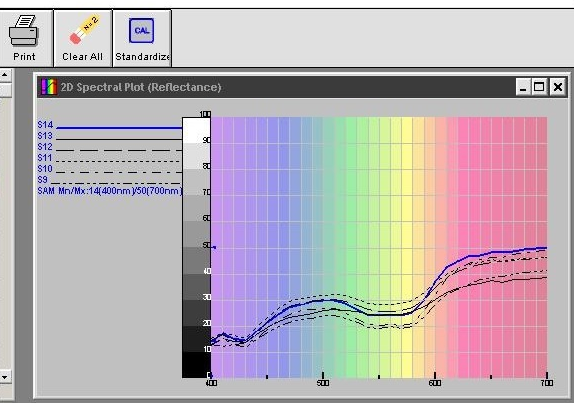
\includegraphics[scale=0.56]{img/HunterLabSoftware}
		\end{figure}
	
		\begin{figure}[H]
			\caption{FIGURA 2. Curva de Reflectancia del software en desarrollo}
			\centering
			\label{figura_1}
			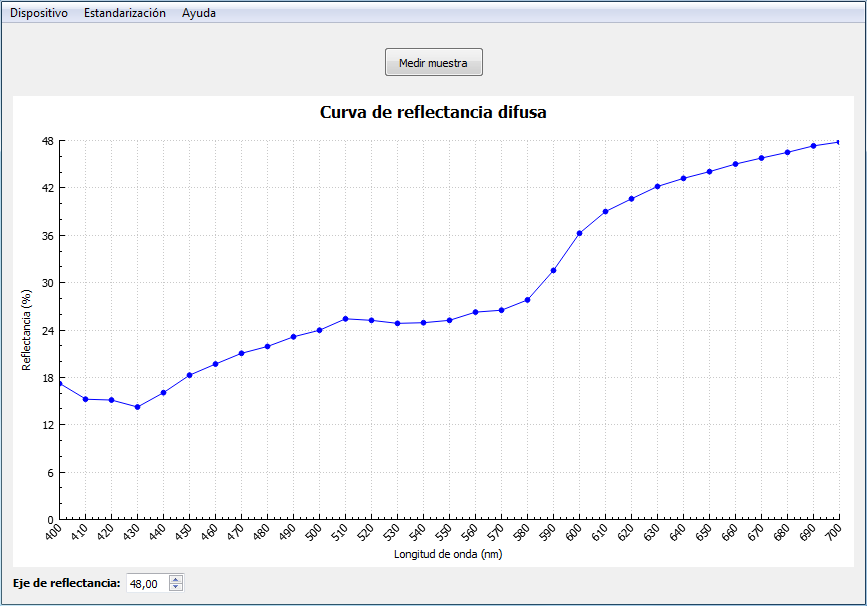
\includegraphics[scale=0.37]{img/nuevoSoftware}
		\end{figure}
	
	\subsection{Conclusiones}
	Si bien el nuevo software est\'{a} en una fase temprana de desarrollo, se puede apreciar que provee de informaci\'{o}n m\'{a}s detallada sobre la Curva de Reflectancia Difusa que el ``HunterLab Universal Software''; no solamente eso, sino que el empleo del Framework Qt para su desarrollo permite su ejecuci\'{o}n en Sistemas Operativos Windows actuales, por lo que se concluye que este software ser\'{a} capaz de ajustarse a las necesidades de los dermat\'{o}logos, y garantizar\'{a} un mejor aprovechamiento del ``MiniScan XE Plus''.
% conference papers do not normally have an appendix

\newpage

% use section* for acknowledgement
\section*{Agradecimientos}
...

% trigger a \newpage just before the given reference
% number - used to balance the columns on the last page
% adjust value as needed - may need to be readjusted if
% the document is modified later
%\IEEEtriggeratref{8}
% The "triggered" command can be changed if desired:
%\IEEEtriggercmd{\enlargethispage{-5in}}

% references section

% can use a bibliography generated by BibTeX as a .bbl file
% BibTeX documentation can be easily obtained at:
% http://www.ctan.org/tex-archive/biblio/bibtex/contrib/doc/
% The IEEEtran BibTeX style support page is at:
% http://www.michaelshell.org/tex/ieeetran/bibtex/
%\bibliographystyle{IEEEtran}
% argument is your BibTeX string definitions and bibliography database(s)
%\bibliography{IEEEabrv,../bib/paper}
%
% <OR> manually copy in the resultant .bbl file
% set second argument of \begin to the number of references
% (used to reserve space for the reference number labels box)
\begin{thebibliography}{1}

\bibitem{Perez}
A.~D. P\'{e}rez, \emph{Estudio de la Reflexi\'{o}n \'{O}ptica Difusa en Tejido Biol\'{o}gico}.\hskip 1em plus
  0.5em minus 0.4em\relax Escuela Superior de Ingenier\'{i}a Mec\'{a}nica y El\'{e}ctrica Unidad Zacatenco, 2012.

\bibitem{Bersha}
K.~S. Bersha, \emph{Spectral Imaging And Analysis Of Human Skin}.\hskip 1em plus
  0.5em minus 0.4em\relax University of Eastern England, 2010.

\bibitem{HunterLab}
Hunter Associates Laboratory, \emph{HunterLab, The World's true measure of color}.\hskip 1em plus
0.5em minus 0.4em\relax http://www.hunterlab.com/about-us.html.

\bibitem{HunterLab-manual}
\emph{Universal Software Versions 4.10 and Above User's Manual}.\hskip 1em plus
  0.5em minus 0.4em\relax Reston, Virginia: Hunter Associates Laboratory, 2001.

\bibitem{Sommerville}
I. Sommerville, \emph{Ingenier\'{i}a del Software}, 7ma~ed.\hskip 1em plus
  0.5em minus 0.4em\relax Madrid, Espa\~{n}a: Pearson Education, 2005.

\bibitem{CIE}
CIE, \emph{Commission Internationale de l'Eclairage, International Commission on Illumination}.\hskip 1em plus
0.5em minus 0.4em\relax http://www.cie.co.at/index.php.

\bibitem{Schanda}
J. Schanda, \emph{Colorimetry: understanding the CIE system}.\hskip 1em plus
  0.5em minus 0.4em\relax Hoboken, New Jersey: John Wiley \& Sons, 2007.

\bibitem{Narea}
F. Narea et al., \emph{Recuperaci\'{o}n del coeficiente de absorci\'{o}n de la epidermis en la piel humana}.\hskip 1em plus
  0.5em minus 0.4em\relax Sociedad Espa\~{n}ola de \'{O}ptica, 2015.

\bibitem{Baskerville}
R.~L. Baskerville, \emph{Investigating Information Systems with Action Research}, vol~2.\hskip 1em plus
  0.5em minus 0.4em\relax Atlanta, GA: Association for Information Systems, 1999.

\bibitem{Schwaber&Sutherland}
K. Schwaber y J. Sutherland, \emph{The Definitive Guide to Scrum: The Rules of the Game}.\hskip 1em plus
  0.5em minus 0.4em\relax http://www.scrumguides.org/.

\bibitem{Kroll&Kruchten}
P. Kroll y P. Kruchten, \emph{The Rational Unified Process Made Easy: A Practitioner's Guide to the RUP}.\hskip 1em plus
  0.5em minus 0.4em\relax Addison-Wesley, 2003.

\bibitem{MiniScanXEPlus-manual}
\emph{MiniScan XE Plus User's Guide Version 2.4}.\hskip 1em plus
  0.5em minus 0.4em\relax Reston, Virginia: Hunter Associates Laboratory, 2006.

\bibitem{RS232}
Magneto Tech Research, \emph{USB to Serial adapters Wiki}.\hskip 1em plus
0.5em minus 0.4em\relax http://www.usb-serial-adapter.org/.

\bibitem{Qt}
The Qt Company, \emph{Qt, a Cross-Platform Framework for Application Development}.\hskip 1em plus
0.5em minus 0.4em\relax https://wiki.qt.io/About\_Qt.

\bibitem{VS}
Microsoft, \emph{Visual Studio Community, a fully-featured, extensible IDE}.\hskip 1em plus
0.5em minus 0.4em\relax https://www.visualstudio.com/products/visual-studio-community-vs

\bibitem{QCustomPlot}
QCustomPlot, \emph{a Qt C++ widget for plotting and data visualization}.\hskip 1em plus
0.5em minus 0.4em\relax http://www.qcustomplot.com/index.php/introduction.

%\bibitem{Pressman}
%R.~S. Pressman, \emph{Ingenier\'{i}a del Software, un enfoque pr\'{a}ctico}, %5ta~ed.\hskip 1em plus
%  0.5em minus 0.4em\relax Madrid, Espa\~{n}a: McGraw Hill, 2002.

\end{thebibliography}

% that's all folks
\end{document}


